%%%%%%%%%%%%%%%%%%%%%%%%%%%%%%%%%%%%%%%
% Hieu Do - Resume
% 7/26/2016
%
% Reference:
% Debarghya Das (http://debarghyadas.com)

\documentclass[]{hieudo-build}
\usepackage[export]{adjustbox}
\usepackage{wrapfig}
\begin{document}
%%%%%%%%%%%%%%%%%%%%%%%%%%%%%%%%%%%%%%
%
%     TITLE NAME
%
%%%%%%%%%%%%%%%%%%%%%%%%%%%%%%%%%%%%%%
%\namesection{\fontsize{30}{10}\selectfont
%Onkar Jagannath Sathe}{}

\namesection{Onkar}{Sathe}
{ +91 9923117590  |  \href{mailto:onkarsathe27@gmail.com}{onkarsathe27@gmail.com }  |  \href{https://www.linkedin.com/in/onkar-sathe/}{linkedin/onkar-sathe}  |  \href{https://github.com/onkar27}{github/onkar27 }}

\begin{minipage}{0.38\textwidth}
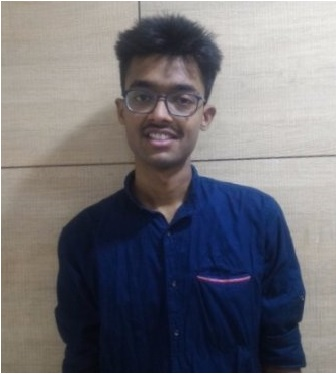
\includegraphics[width=.5\linewidth]{profile.jpg}

%%%%%%%%%%%%%%%%%%%%%%%%%%%%%%%%%%%%%%
%     EDUCATION
%%%%%%%%%%%%%%%%%%%%%%%%%%%%%%%%%%%%%%

\section{Education}
\subsection{Walchand College of Engineering}
\descript{B.Tech in Computer Science and Technology}
Sangli | Expected Grad. May 2019 \\
CPI : 8.0\\
\sectionsep

\subsection{Shri. Shivaji Mahavidyalaya}
\descript{Higher Secondary (H.S.C)} Barshi | 2014 - 2015 \\
Percentage : 82.42 %\\
\sectionsep

\subsection{Sulakhe High School}
\descript{Secondary (S.S.C)} Barshi | 2012 - 2013 \\
Percentage : 93.45 %\\

\sectionsep
%%%%%%%%%%%%%%%%%%%%%%%%%%%%%%%%%%%%%%
%     SKILLS
%%%%%%%%%%%%%%%%%%%%%%%%%%%%%%%%%%%%%%

\section{Technical Skills}
\subsection{Programming Languages:}
\begin{tabular}{lll}
\textbullet{ C } &\textbullet{ C++} &\textbullet{ Python}\\
\textbullet{ Java } &\textbullet{ SQL} &\textbullet{ Javascript}\\
\end{tabular}

\subsection{Techonologies :}
\begin{tabular}{lll}
\textbullet{ Django } &\textbullet{ JavaFX } &\textbullet{ Android }
\end{tabular}

\section{Soft Skills}
\textbullet{ Good teamwork abilities } \\
\textbullet{ Curious and hardworking } \\
\textbullet{ Quick grasping }

\sectionsep
%%%%%%%%%%%%%%%%%%%%%%%%%%%%%%%%%%%%%%
%     COURSEWORK
%%%%%%%%%%%%%%%%%%%%%%%%%%%%%%%%%%%%%%
\section{Coursework}
\textbullet{ Data Structure } \\
\textbullet{ Database System } \\
\textbullet{ Design and Analysis of Algorithms} \\
\textbullet{ Image Processing}\\
\textbullet{ Operating System}\\
\sectionsep

\end{minipage}
\begin{minipage}{0.6\textwidth}
\section{Objective}
\descript{Seeking a summer internship with the e-Yantra where my strong analytical and problem solving skills will be utilized and passionately develop myself while helping the community. }

\sectionsep
%%%%%%%%%%%%%%%%%%%%%%%%%%%%%%%%%%%%%%
%     EXPERIENCE
%%%%%%%%%%%%%%%%%%%%%%%%%%%%%%%%%%%%%%
\section{Experience}

\workplace{WCE - ACSES | Programming Expert}{Jan 2018 – present}\\
\descript{
- Problem Setter for monthly coding contests
}

\sectionsep

%%%%%%%%%%%%%%%%%%%%%%%%%%%%%%%%%%%%%%
%     Achievements
%%%%%%%%%%%%%%%%%%%%%%%%%%%%%%%%%%%%%%
\section{Achievements}
\workplace{2nd Runner-up eYantra Robotics Competition 2018}{IITB} \\
\descript {
- Real-world problems assigned as "themes" by IITB are then implemented using the robotic kits  and demonstrated at IIT Bombay. }
\sectionsep

\workplace{Barclays Hackathon 2018}{Pune} \\
\descript {
- "Best Male Coder Award" \\
- Finalist : Barclays Hackathon 2018 to solve real-world problems with scalable solutions and secured position among top 20 teams from 1908.}
\sectionsep

\workplace{ACM ICPC 2017}{Kolkata-Kanpur} \\
\descript {Represented Walchand College of Engineering Sangli at ACM-ICPC \\
- It knows where talk about tour competitive programming profiles and stood 65th Rank among 168 teams.}

\sectionsep
%%%%%%%%%%%%%%%%%%%%%%%%%%%%%%%%%%%%%%
%     PROJECTS
%%%%%%%%%%%%%%%%%%%%%%%%%%%%%%%%%%%%%%
\section{Projects}
\runsubsection{Codedaemon}
\descript{| Online Judge |
{\href{https://github.com/onkar27/CODEDAEMON}{ LINK }}}
\sectionsep
\begin{tightemize}
\item  Conducted 6 competitions successfully with average signup count of 40 and support [ Python, Java, C++, C ] languages.
\end{tightemize}
\vspace{1pt}

\runsubsection{BillDesk Invoicing}
\descript{| Billing System and Sales Predictions for Kirana stores}
\begin{tightemize}
\item  Sales predicted will be based on the past training data of sales using machine learning.
\item Sending bills via mail, SMS to introduce paperless billing.
\end{tightemize}
\vspace{1pt}

\runsubsection{Eyantra Robotics Competition}
\descript{| e-YRC 2017 - Theme: Collector Bot }
\begin{tightemize}
\item Automatic bot is designed to collect fresh fruits.
\item Identifying shapes of objects, color, and nearest matching object and path between them, using image processing.
\end{tightemize}

\runsubsection{QuickTransfer}
\descript{| A java based file transfer software. |{\href{https://sourceforge.net/projects/darkeye-quicktransfer/}{ LINK }}}

\begin{tightemize}
\item A PC-to-PC File sharing software which provides User Friendly GUI, Multiple Files Sharing, End to End Encryption
\item ‘Share Me’ Feature – Quick Transfer Web.
\end{tightemize}

\runsubsection{ Event Scheduling}
\runsubsection{\textbullet{ JCodeIt}}
\runsubsection{\textbullet{ Text Compression Software}}
\end{minipage}
\noindent
\\

%%%%%%%%%%%%%%%%%%%%%%%%%%%%%%%%%%%%%%
%     Extra-Curricular activities
%%%%%%%%%%%%%%%%%%%%%%%%%%%%%%%%%%%%%%
\section{Extra-Curricular activities}
\workplace{SITAC - ACSES | Volunteer }{Feb 2018}\\
\descript{
- Social IT Awareness Camp (SITAC) is camp conducted by ACSES , WCE , Sangli every year to make the children of nearby schools aware about the knowledge of Computer Science and the upcoming technologies.
}
\sectionsep
\workplace{CodeWizard - Techumen  | Event Head }{Oct 2017}\\
\descript{
- Lead as event head in national coding event
}
\sectionsep
\descript{ - Finalist : Hindustan Unilever Limited HACKATHON | 2017.\\
 - Finalist : Debugging Competition COEP's Mindspark.\\
 - 2nd Runner-up : Reverse Coding Competition held by PICT 2016.\\
 - 3 Silvers and 9 Bronze : Hackerrank Rated contests. LINK:  \href{https://www.hackerrank.com/os1997}{\custombold{ os1997 }} \\
 - 3 Stars [ 1766 ] CodeChef Rating  LINK:\href{https://www.codechef.com/users/onkar27}{\custombold{ onkar27 }}
}

\sectionsep
\section{Personal Information}
\descript{ Father's Name : Jagannath Ambu Sathe\\
Mother's Name : Rekha Jagannath Sathe\\
Sex :	Male\\
Date of Birth : 31-Aug-1997\\
Nationality : Indian\\
Marital Status : unmarried
}
\sectionsep
\section{Hobbies}
\descript{
Competitive Coding\\
Traveling\\
Listening Music
}
\sectionsep
\subsection{Reference}
\href{https://github.com/lohitpenu/Internship-eYSIP-2018}{https://github.com/lohitpenu/Internship-eYSIP-2018}\\
\href{https://www.overleaf.com}{https://www.overleaf.com}

\sectionsep
\subsection{Declaration}
\descript{I hereby declare that the above information is correct to the best of my knowledge.}

\sectionsep
\sectionsep{Date : 18 April 2018}
\end{document}
